\documentclass[letter,12pt]{article}
\usepackage{inputenc}
\usepackage{mdframed}
%\usepackage{minted}[linenos=true,frame=single,framesep=2mm,baselinestretch=1.2]
\usepackage{minted}[
frame=single,
framesep=2mm,
baselinestretch=1.2,
bgcolor=blue,
linenos]
\usepackage{graphicx}
\usepackage{subcaption}
\usepackage{float}
\usepackage[toc]{appendix}
\BeforeBeginEnvironment{minted}{\begin{mdframed}}
\AfterEndEnvironment{minted}{\end{mdframed}}

\title{Using Single Port RAM on a Cyclone V}
\author{Liam Ramsey}

\begin{document}

\maketitle

\section{Adding the RAM to Your Project}
There are two ways you can add the RAM to your Quartus project, either with the IP Catalog or by writing it in by hand.

\subsection{Using the IP Catalog}

If you do not already have the IP Catalog open in Quartus, you can get to it by going to Tools$\rightarrow$IP Catalog. From the IP Catalog you can go to Library$\rightarrow$Basic Functions$\rightarrow$On Chip Memory and double click RAM: 1-PORT. This opens the megafunction wizard for the module.

\begin{figure}[h!]
  \centering
  \begin{subfigure}[b]{0.4\linewidth}
    \centering
    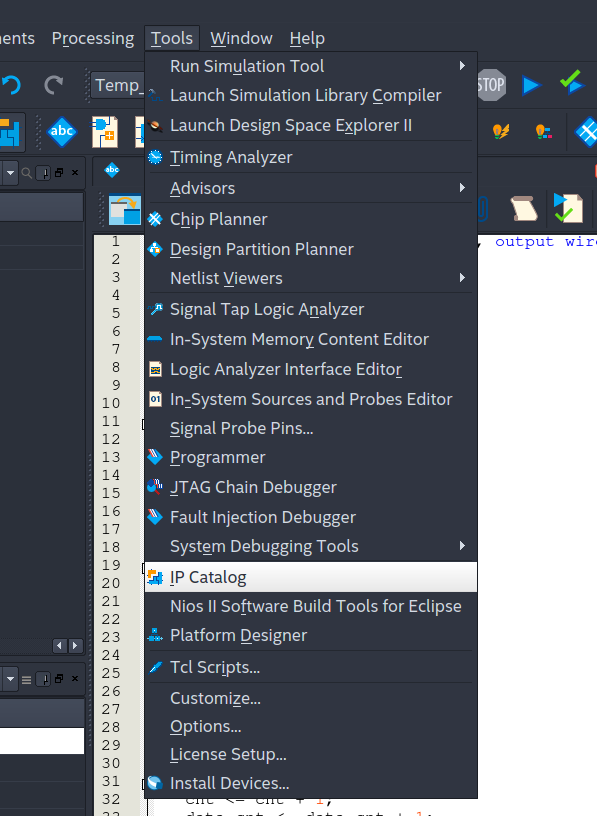
\includegraphics[width=0.75\linewidth]{pics/IPCatalog.png}
    \caption{IP Catalog}
  \end{subfigure}
  \begin{subfigure}[b]{0.4\linewidth}
    \centering
    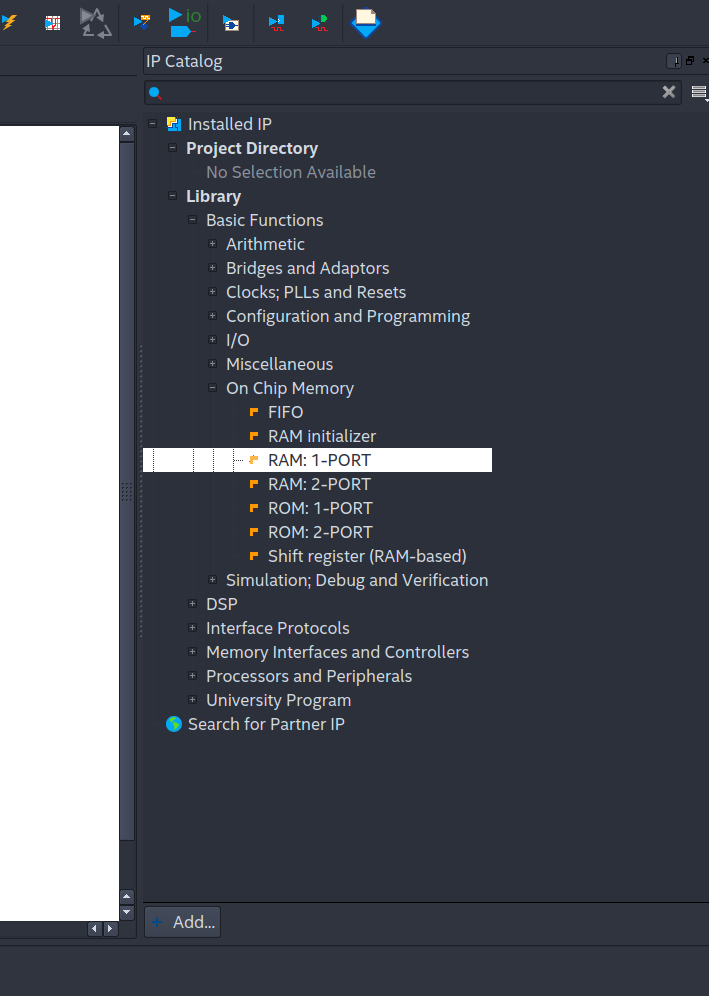
\includegraphics[width=0.75\linewidth]{pics/RAM1Port.png}
    \caption{RAM: 1-PORT}
  \end{subfigure}
  \caption{}
\end{figure}

With the megafunction wizard open, you can specify the size in bits stored at each memory address by setting the width of the output bus ``q''. Setting how many words of memory specifies how many addresses we have to use, so total memory capacity will be number of words times how many bits per word. Leaving the rest to ``Auto'' and ``Single clock'' are fine, unless you know you need otherwise.

\begin{figure}[H]
  \centering
  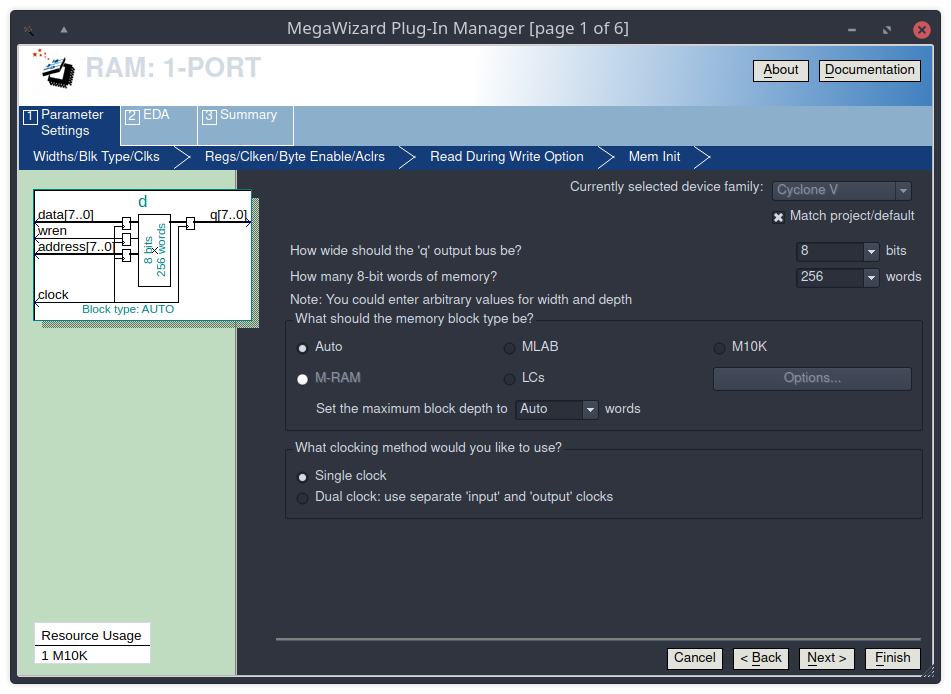
\includegraphics[width=.83\linewidth]{pics/Mega1.png}
  \caption{MegaWizard page 1}
\end{figure}

For pages 2 and 3 options can be left at default for a simple implementation. Things to note are the addition of an  all clear signal and a read enable signal. 
\begin{figure}[H]
  \centering
  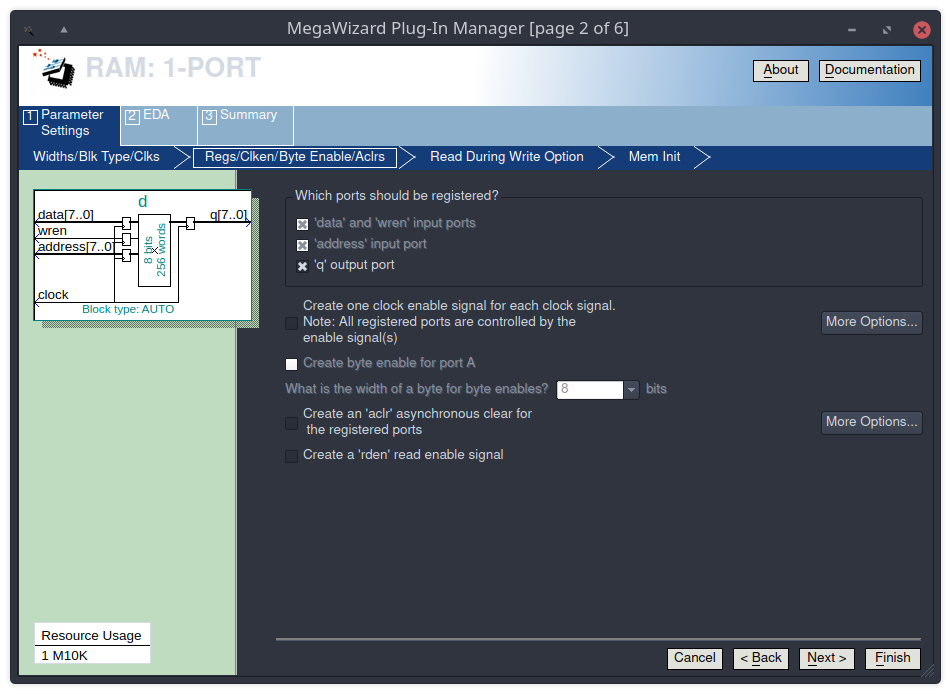
\includegraphics[width=.83\linewidth]{pics/Mega2.png}
  \caption{MegaWizard page 2}
\end{figure}
\begin{figure}[H]
  \centering
  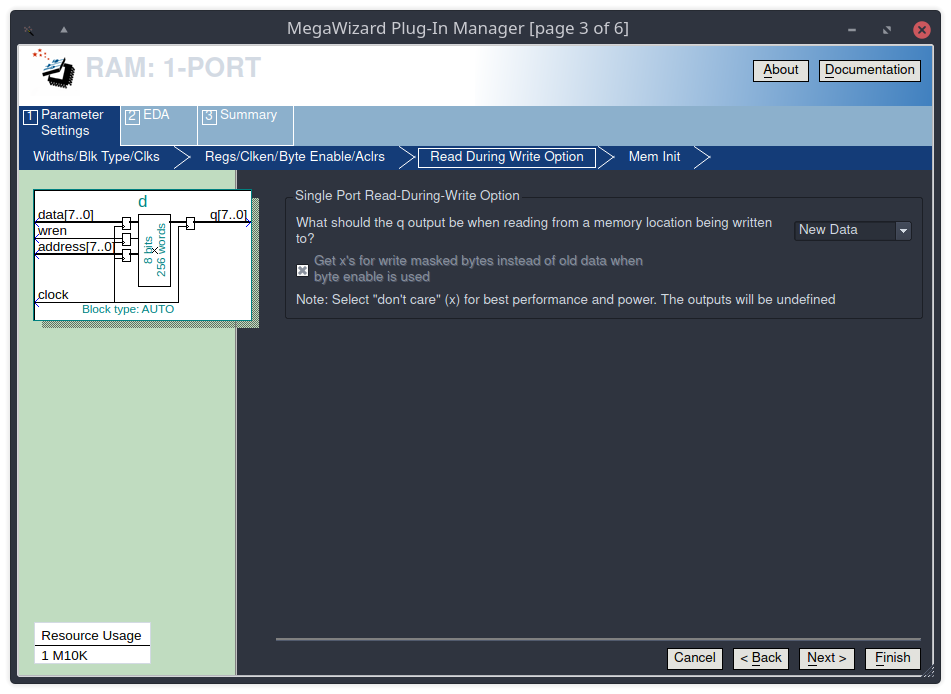
\includegraphics[width=.83\linewidth]{pics/Mega3.png}
  \caption{MegaWizard page 3}
\end{figure}

On page 4 here you'll want to check the box for ``Allow In-System Memory Content Editor ...'' so that the memory is accessable by external means. Here you can also specify initial contents of the memory. A .mif file can be generated using the mif python package.

\begin{figure}[H]
  \centering
  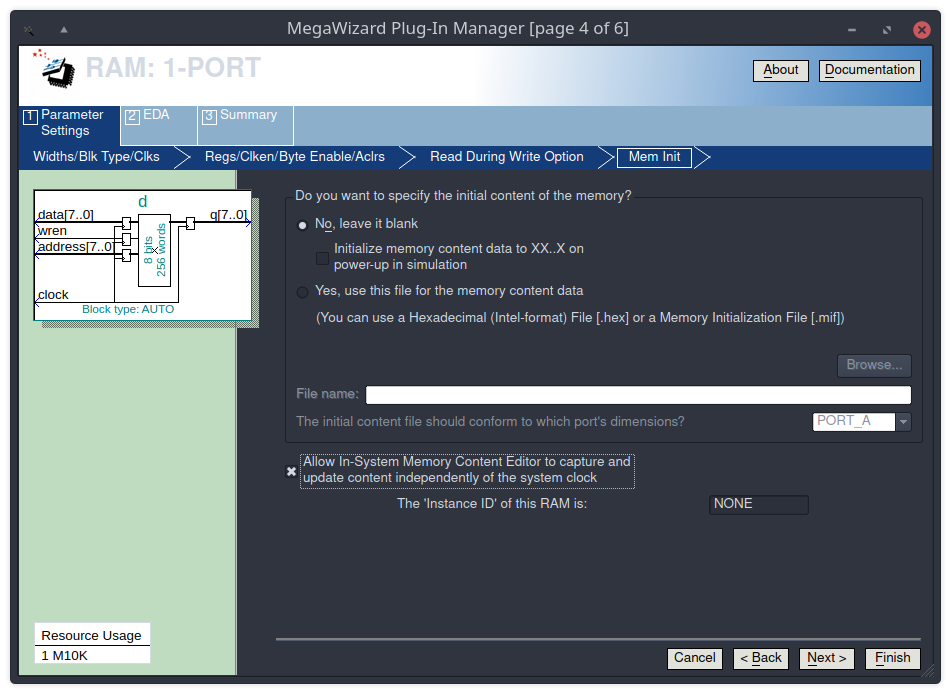
\includegraphics[width=.83\linewidth]{pics/Mega4.png}
  \caption{MegaWizard page 4}
\end{figure}
\begin{figure}[H]
  \centering
  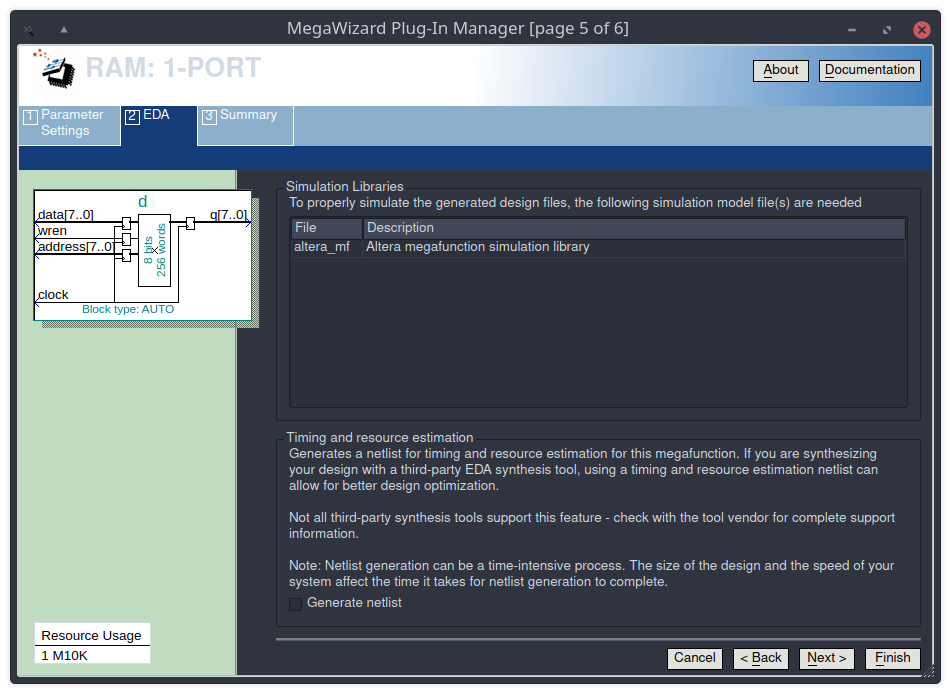
\includegraphics[width=.83\linewidth]{pics/Mega5.png}
  \caption{MegaWizard page 5}
\end{figure}

Here you can define which files Quartus will generate for you. The main \textless name\textgreater.v and \textless name\textgreater\_bb.v files are checked by default. Additionally Quartus can generate \textless name\textgreater\_inst.v, which contains an example if instantiating the module, you do not need to select this, as I will provide instantiation code here.
After clicking finish, Quartus will prompt you to add the IP to your project.

\begin{figure}[H]
  \centering
  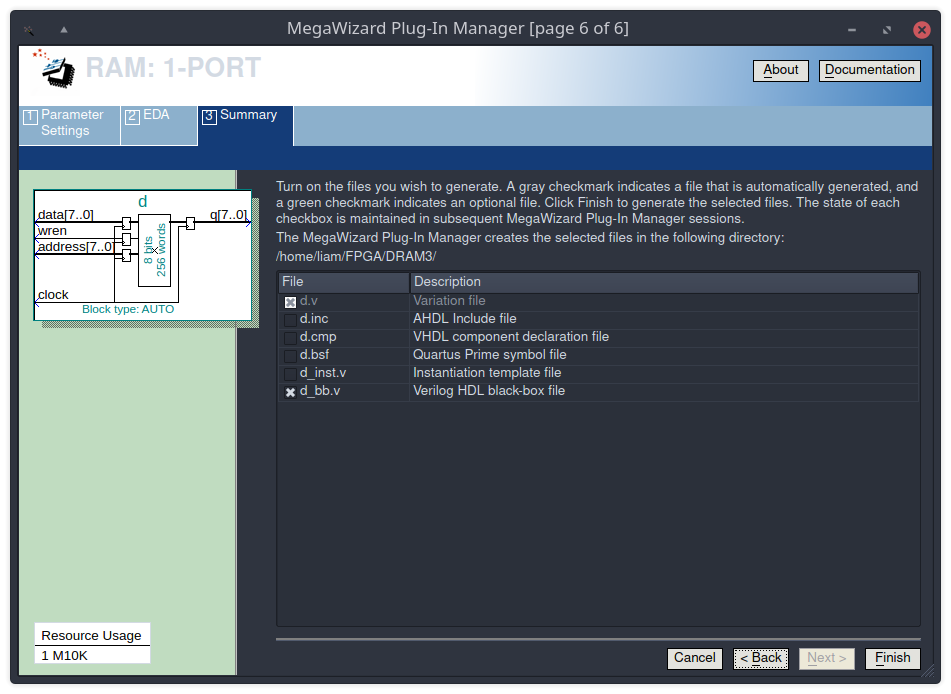
\includegraphics[width=.83\linewidth]{pics/Mega6.png}
  \caption{MegaWizard page 6}
\end{figure}

%\subsection{Using the altsyncram primitive}
%TODO: Figure out Noelo's verilog.

\section{Using the Memory}
\subsection{Instantiating the module and writing to it}

The memory can be instantiated with the following verilog. Something important to note, instantiating multiple times from the same IP will create multiple RAM instances with different indices but the same instance ID name (See the columns in the In-System Memory content editor). This is important to keep in mind when using the python interface as the find\_instance function will only find one of them.

\begin{minted}[linenos=true]{verilog}
<name> ram_inst (
    .address ( address_sig ),
    .clock ( clock_sig ),
    .data ( data_sig ),
    .wren ( wren_sig ),
    .q ( q_sig )
);
\end{minted}

You need to define the inputs and outputs earlier in the code with the names in the parentheses. Also replace \textless name\textgreater\ with the name that you assigned the IP module. The register sizes must match the values specified when the module was created. For example the declarations for a RAM module with 8-bit words and a 8-bit address space would be:

\begin{minted}[linenos=true]{verilog}
reg address_sig[7:0];
reg data_sig[7:0];
wire wren_sig;
wire clk_sig;
reg q_sig[7:0];

assign clk_sig = clk;
\end{minted}

Where clk is the input clock to your main module, and \textless name\textgreater is the name given to the RAM module. To write a value to memory, first the wren\_sig wire must be set high (you could assign a register to it), then the desired values need to be put into the address\_sig and data\_sig registers. For an example of a complete verilog file see Appendix B.

%Some thought needs to be given to the TODO: Document undefined behavior in single clock cycles.

\subsection{Interfacing With the Memory Using the In-System Memory Content Editor}

The simplest way to read and write to the memory on the FPGA is to use Quartus's In-System Memory Content Editor. However, more functionality can be achieved by using the Python packaged described in the next section.

\begin{figure}[H]
  \centering
  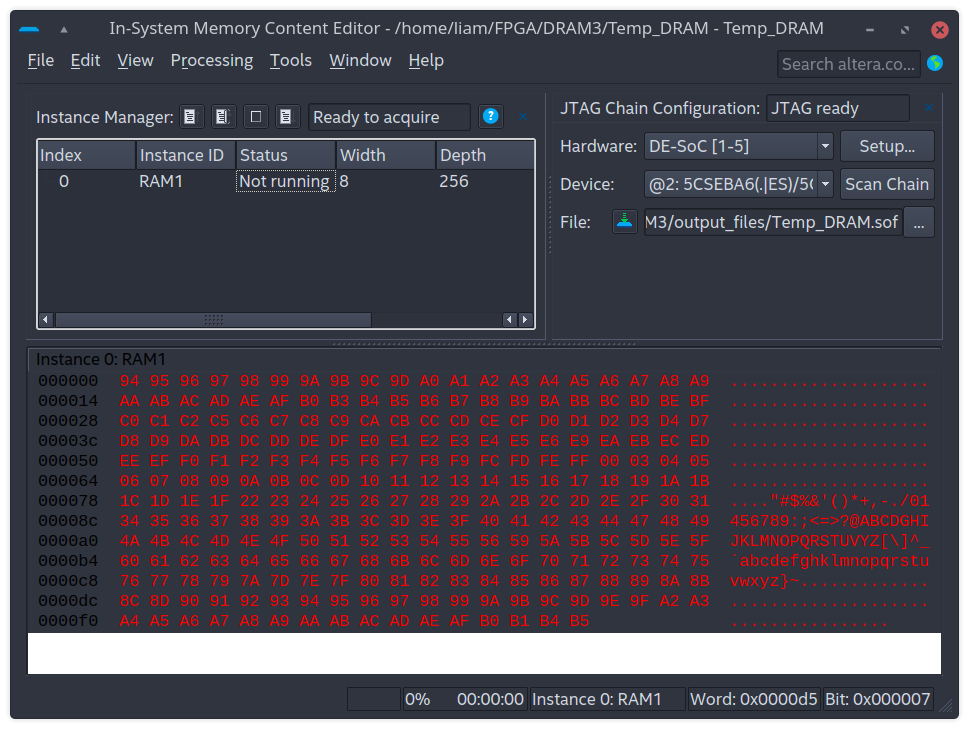
\includegraphics[width=\linewidth]{pics/MemoryEditor.png}
  \caption{In-System Memory Content Editor}
\end{figure}

In the upper right section of the window, we have the basic functionality of the device programmer. Clicking the button directly to the right of ``File:'' will program the FPGA with the specified .sof file. The top left section lists the memory instances Quartus has found on the board. Right clicking an instance provides different options to read and write to the memory. The bottom section contains the memory currently selected in hex values on the left, and ASCII decoded on the right.

\subsection{Using the mif and quartustcl Python Packages}

In order to interface with the memory using these packages we will be using the QuartusMemory class. In order to use the quartustcl package that QuartusMemory is based on in Windows, you must add the quartus scripts to your environment path variable. This can be done by first locating the quartus install directory, typically at C:\textbackslash IntelFPGA\_lite\textbackslash\textless version\textgreater\textbackslash quartus\textbackslash bin64. This needs to be added to the PATH environment variable. This can be done by windows searching for ``Environment Variables'' and editing the path variable as shown below.

\begin{figure}[H]
  \centering
  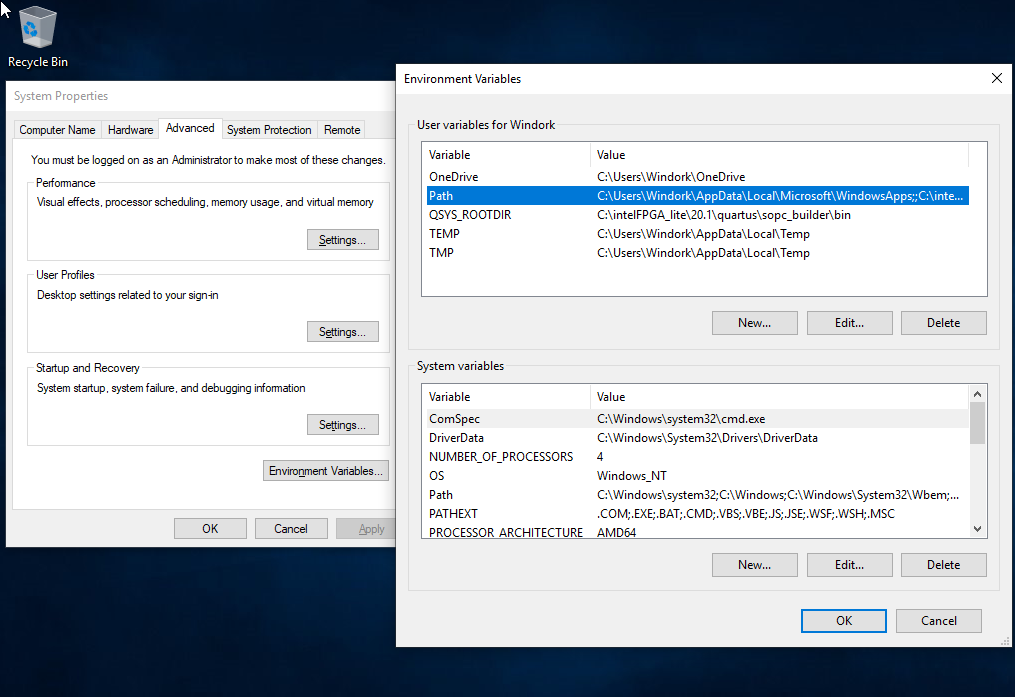
\includegraphics[width=\linewidth]{pics/EnvironmentVariables.png}
  \caption{Editing the PATH environment variable}
\end{figure}

With this done, quartus scripts can now be used via command line and the python package quartustcl will function. Code for the QuartusMemory class is provided in Appendix A. Below is an example program using the class.

\begin{mdframed}
\inputminted[linenos=true,breaklines,breakanywhere=true]{python}{../../Python/memoryExample.py}
\end{mdframed}

The code here simply reads the memory from the device into an array, changes a bit in it, writes it back to the device, then lastly reads to confirm the write executed correctly. The boolean argument at the end of each function call is whether to delete the .mif file generated. Both read and write default to not delete it. It is worth noting that running this script multiple times will overwrite and delete previously generated .mif files. If saving them is desired they should be renamed. The array format is of a two dimensional numpy array consisting of 1's and 0's with type uint8 (unsigned 8-bit integer). This code can be found at https://github.com/Noeloikeau/TDC/tree/Liam in the Python folder.

\newpage
\appendix

\section{QuartusMemory Python Class}

Code for the QuartusMemory class. Also available at \\ https://github.com/Noeloikeau/TDC/tree/Liam in the Python folder.

\begin{mdframed}
\inputminted[linenos=true,breaklines,breakanywhere=true]{python}{../../Python/QuartusMemory.py}
\end{mdframed}

\section{Verilog Example}
An example of a 1-Port RAM module being filled with the output of a counter.

\begin{mdframed}
\inputminted[linenos=true,breaklines,breakanywhere=true]{verilog}{memExample.v}
\end{mdframed}

\end{document}

